\documentclass{beamer}
\mode<presentation>
{
\usetheme{Darmstadt}
%\usecolortheme{crane} %yellow
%%% BYU colored theme
\definecolor{BYUBlue}{RGB}{00,22,55}
\definecolor{BYUTan}{RGB}{232,211,175}
\usecolortheme[named=BYUBlue]{structure}
\setbeamercolor*{palette primary}{use=structure,fg=BYUBlue,bg=lightgray}
\setbeamercolor*{palette quaternary}{fg=white,bg=lightgray!0!BYUBlue}
\setbeamercolor{frametitle}{fg=BYUBlue,bg=BYUBlue!10}
\setbeamertemplate{items}[circle]
\setbeamertemplate{blocks}[rounded][shadow=True]
\setbeamertemplate{navigations symbols}{circle}
}

\usepackage{graphics}
\usepackage[english]{babel}
\usepackage[utf8]{inputenc}
\usepackage{times}
\usepackage[T1]{fontenc}
\usepackage{array}
\usepackage{amsmath,amssymb}
\usepackage{colortbl}
\usepackage{listings}
\usepackage{array}
\usepackage{threeparttable}
\usepackage{multirow}
\usepackage{amsthm}
\usepackage{float,graphicx,color}
\usepackage{graphics}
\usepackage{multicol}
\usepackage{natbib}
\usepackage{color}
\usepackage{hyperref}
\hypersetup{colorlinks, urlcolor=blue}
\usepackage{threeparttable}
\usepackage[format=hang,font=normalsize,labelfont=bf]{caption}
\usepackage{subcaption}
\usepackage{delarray}
\usepackage{amssymb}
\usepackage{setspace}
%\usepackage[pdftex]{graphicx}
\usepackage{placeins}
\usepackage{multirow}
\usepackage{mathtools}
\usepackage{animate}
\usepackage{bm}
\newcommand\ve{\varepsilon}
\newcommand\norm[1]{\left\lVert#1\right\rVert}

\title[Title]{US Covert Operations and Suicide Terrorism}

%\subtitle
%{} % (optional)

\author[Yourname]{\textbf{Soo Wan Kim}}
% - Use the \inst{?} command only if the authors have different
%   affiliation.

\date[Short Occasion]{April 5, 2017}

% This section of code puts a slide showing where you are in the outline
% at the beginning of each section
% \AtBeginSection[]
% {
%  \begin{frame}<beamer>{Outline}
%   \tableofcontents[currentsection]
%   %\tableofcontents[currentsection, subsection]
%  \end{frame}
% }


% If you wish to uncover everything in a step-wise fashion, uncomment
% the following command:

%\beamerdefaultoverlayspecification{<+->}


\begin{document}

\begin{frame}
  \titlepage
\end{frame}

\section{Introduction}

  \begin{frame}
    \frametitle{Introduction}
	\begin{block}{Covert Operation}
"An operation that is so planned and executed as to conceal the identity of or permit plausible denial by the sponsor." 
\\
\footnotesize(U.S. Department of Defense Dictionary of Military and Associated Terms)
\\
\vspace{2mm}
\small Generally speaking: drone strikes, other air strikes
    \end{block}
    \begin{itemize}
      \item The Obama administration relied heavily on drone strikes and other covert operations to target the leadership of terrorist groups
	\item These operations allow the US to reduce their military footprint overseas, but attract international controversy due to collateral damage to civilians and their secretive nature
    \end{itemize}
  \end{frame}

  \begin{frame}
	\begin{figure}[h!]
		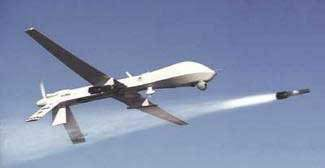
\includegraphics[width=\linewidth]{Predator_and_Hellfire.jpg}
	\end{figure}
  \end{frame}

  \begin{frame}
	\begin{figure}[h!]
		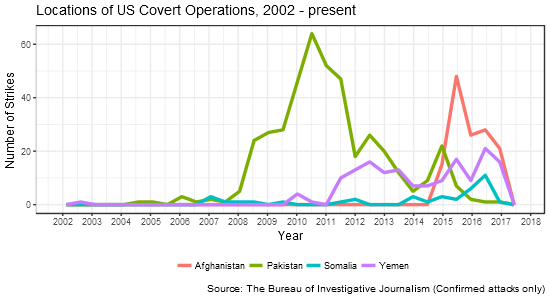
\includegraphics[width=\linewidth]{combined_strikes.png}
	\end{figure}
  \end{frame}

  \begin{frame}
    \frametitle{Research Question}
    \begin{itemize}
      \item Do covert US air strikes delay or hasten subsequent suicide terrorist bombings in the countries where the strikes are carried out?
    \end{itemize}
  \end{frame}

\section{Literature Review}

  \begin{frame}
    \frametitle{Theory}
    \begin{itemize}
       \item Scholars divided on the utility of air strikes in counter-terrorism
	\item Rival sets of theories:
		\begin{itemize}
			\item \textbf{Blowback/Backlash}: Strikes anger local populations and increase support for terrorist groups $\rightarrow$ more terrorism
			\item \textbf{Disruption, degradation, deterrence}: Strikes interfere with terrorist groups' operations, remove key players, and deter would-be terrorists $\rightarrow$ less terrorism
		\end{itemize}
\end{itemize}
  \end{frame}

  \begin{frame}
    \frametitle{Empirical Findings: Incidence Models}
	\begin{figure}[h!]
		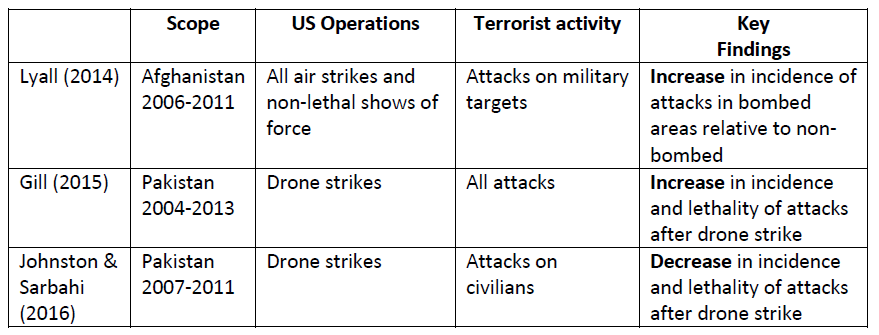
\includegraphics[width=\linewidth]{incidence_models.PNG}
	\end{figure}
  \end{frame}

 \begin{frame}
    \frametitle{Gaps in the Literature (1)}
	\begin{itemize}
		\item Which types of terrorism are relevant? Not all acts are carried out by the groups targeted in US air strikes. Some carried out by rival groups or lone wolves. Impossible to know for certain who committed what. Thus, looking at terrorist activity as a whole may not be helpful for gauging the effect of air strikes on the groups they specifically target.
	\end{itemize}
\vspace{3mm}
    \begin{alertblock}<2->{Proposed solution}
      Use suicide bombings only. Suicide bombings are particularly difficult to carry out, require heavy explosives and often specific training. They are the hallmark of professional terrorist cells, not lone wolves. Also, they are widely used by the groups targeted in US air strikes.
    \end{alertblock}
  \end{frame}

 \begin{frame}
    \frametitle{Gaps in the Literature (2)}
	\begin{itemize}
		\item Do air strikes hasten or delay terrorist activity? Looking at the incidence of attacks across a longer period (e.g. month) does not answer this question because attacks can be spaced closely together or far apart.
	\end{itemize}
\vspace{3mm}
    \begin{alertblock}<2->{Proposed solution}
      Look at the length of time between attacks.
    \end{alertblock}
  \end{frame}

\section{Data \& Methods}

  \begin{frame}
    \frametitle{Question \& Hypotheses}
    \begin{itemize}
	\item \textbf{Research question (restated)}: Do covert US air strikes delay or hasten subsequent suicide terrorist bombings in the countries where the strikes are carried out?
	\begin{itemize}
		\item \textbf{H1 (Blowback/Backlash)}: Terrorist groups behave more aggressively after an air strike and carry out more attacks in quicker succession.
		\item \textbf{H2 (Disruption/Degradation/Deterrence)}: Terrorist groups are hindered by the effects of air strikes and take longer to prepare and carry out attacks.
	\end{itemize}
     \end{itemize}
  \end{frame}

  \begin{frame}
    \frametitle{Assumptions}
    \begin{itemize}
	\item The effects of drone strikes are not necessarily localized, i.e. terrorist cells may move away from zones targeted by air strikes, or the same terrorist group may respond to an air strike in one part of the country by carrying out an attack in another part of the country. However, they should generally operate in the same country over the short term.
	\item Terrorist groups do not distinguish between different types of air strikes.
     \end{itemize}
  \end{frame}

  \begin{frame}
    \frametitle{Analysis}
    \begin{itemize}
	\item \textbf{Method}: Survival/event history model
	\item \textbf{Unit of analysis}: Country-week
        \item \textbf{Independent variable}: Number of US air strikes (lagged or weighted)
	\item \textbf{Dependent variable}: length of time between individual suicide bombings
     \end{itemize}
  \end{frame}

  \begin{frame}
    \frametitle{Data}
    \begin{itemize}
	\item \textbf{Countries}: Yemen, Somalia, Pakistan, Afghanistan
	\item \textbf{Years}: 2002-2016
	\item \textbf{Drone strikes data}: The Bureau of Investigative Journalism
		\begin{itemize}
			\item Independent watchdog
			\item Data based on international and domestic media reports, government reports and other accounts
			\item Data publicly available for free
			\item Only source for air strikes in all four countries
		\end{itemize}
	\item \textbf{Suicide terrorism data}: UChicago's Suicide Attack Database
		\begin{itemize}
			\item Based on international and domestic media reports
			\item Publicly available, free
		\end{itemize}
     \end{itemize}
  \end{frame}

  \begin{frame}
	\begin{figure}[h!]
		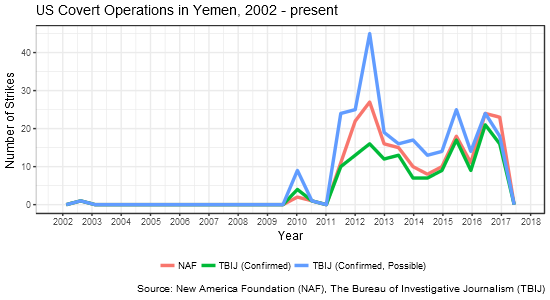
\includegraphics[width=\linewidth]{yemen_strikes.png}
	\end{figure}
  \end{frame}

  \begin{frame}
	\begin{figure}[h!]
		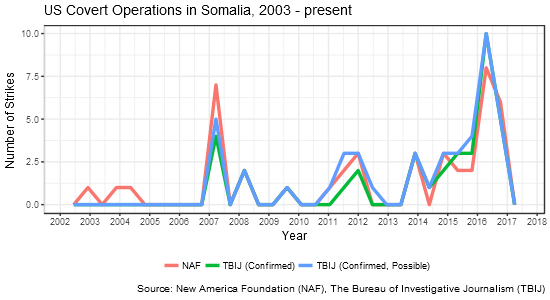
\includegraphics[width=\linewidth]{somalia_strikes.png}
	\end{figure}
  \end{frame}

 \begin{frame}
	\begin{figure}[h!]
		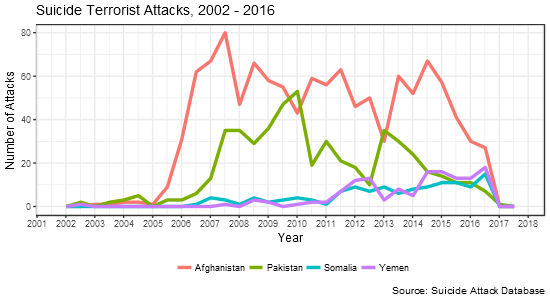
\includegraphics[width=\linewidth]{suicide_attacks.png}
	\end{figure}
  \end{frame}

\section{References}

 \begin{frame}
    \begin{itemize}
	\item Gill, Paul. 2015. “The Impact of Drone Attacks on Terrorism: The Case of Pakistan.” London: Remote Control Project. http://remotecontrolproject.org/wp-content/uploads/2015/06/Paul\_Gill\_drones\_terrorism\_Pakistan.pdf.
	\item Johnston, Patrick B., and Anoop K. Sarbahi. 2016. “The Impact of US Drone Strikes on Terrorism in Pakistan.” International Studies Quarterly 0: 1–17. doi:10.1093/isq/sqv004.
        \item Lyall, Jason. 2014. “Bombing to Lose? Airpower and the Dynamics of Violence in Counterinsurgency Wars.” http://dx.doi.org/10.2139/ssrn.2422170.
     \end{itemize}
  \end{frame}

\end{document}
